\subsection{\RU{Пример с двумерным массивов}\EN{Two-dimensional array example}}

\EN{We are going to work with an array of type \Tchar, which implies that each element requires only one 
byte in memory.}
\RU{Мы будем работать с массивом типа \Tchar. Это значит, что каждый элемент требует
только одного байта в памяти.}

\subsubsection{\RU{Пример с заполнением строки}\EN{Row filling example}}
\index{\olly}

\RU{Заполняем вторую строку значениями}\EN{Let's fill the second row with these values} 0..3:

\lstinputlisting[caption=\RU{Пример с заполнением строки}\EN{Row filling example}]{patterns/13_arrays/5_multidimensional/two1.c.\LANG}

\RU{Все три строки обведены красным}\EN{All three rows are marked with red}. 
\RU{Видно, что во второй теперь имеются байты}\EN{We see that second row now has values} 0, 1, 2 \AndENRU 3:

\begin{figure}[H]
\centering
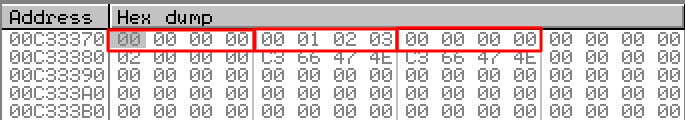
\includegraphics[scale=\NormalScale]{patterns/13_arrays/5_multidimensional/olly_2D_1.png}
\caption{\olly: \RU{массив заполнен}\EN{array is filled}}
\end{figure}

\subsubsection{\RU{Пример с заполнением столбца}\EN{Column filling example}}
\index{\olly}

\RU{Заполняем третий столбец значениями}\EN{Let's fill the third column with values:} 0..2:

\lstinputlisting[caption=\RU{Пример с заполнением столбца}\EN{Column filling example}]{patterns/13_arrays/5_multidimensional/two2.c.\LANG}

\RU{Здесь также обведены красным три строки}\EN{The three rows are also marked in red here}. 
\RU{Видно, что в каждой строке, на третьей позиции, теперь записаны}
\EN{We see that in each row, at third position these values are written:} 0, 1 \AndENRU 2.

\begin{figure}[H]
\centering
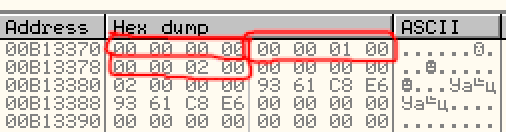
\includegraphics[scale=\NormalScale]{patterns/13_arrays/5_multidimensional/olly_2D_2.png}
\caption{\olly: \RU{массив заполнен}\EN{array is filled}}
\end{figure}
